\documentclass[]{article}
\usepackage{graphicx}
\usepackage{amssymb}
\usepackage{amsmath}
\usepackage{framed}
\usepackage{subcaption}
\usepackage{algorithm}
\usepackage{algpseudocode}
\usepackage{array}
\usepackage{multirow}
\usepackage[hidelinks]{hyperref}
\usepackage{fullpage}
\usepackage{listings}
\lstset{frame=single}
\usepackage{mathtools}
\usepackage{afterpage}

%% tikz 
\usepackage{tikz}
\usetikzlibrary{calc}
\usetikzlibrary{patterns}
\usetikzlibrary{positioning}
\usetikzlibrary{decorations.markings}

% Text
\newcommand{\etc}{etc.}
\newcommand{\eg}{e.g.}
\newcommand{\ie}{i.e.} 

% Math
\newcommand{\sgn}{\operatorname{sign}}
\def\bm#1{\mbox{\boldmath{$#1$}}}
% less space around parentheses 
\let\originalleft\left
\let\originalright\right
\renewcommand{\left}{\mathopen{}\mathclose\bgroup\originalleft}
\renewcommand{\right}{\aftergroup\egroup\originalright}

\title{A guide to writing your first CFD solver} 
\author{Mark Owkes\\ mark.owkes@montana.edu}

\begin{document}
\lstset{language=Matlab}

\maketitle

  \begin{abstract}
  CFD is an exciting field today!  Computers are getting larger and faster and are able to bigger problems and problems at a finer level.  This document provides a guide for the beginners in the field of CFD.  It describes the steps necessary to write a two-dimensional flow solver which can be used to solve the Navier-Stokes equations.  The document begins by reviewing the governing equations and then discusses the various components needed to form a simple CFD solver.
  \end{abstract}

  \tableofcontents
 
\section{Governing equations}
The Navier-Stokes equations describe almost all the flows around us and are the starting point for a CFD code. Additionally since the majority of flows can be approximated as incompressible, we will solve the incompressible form of the equations.  The incompressible Navier-Stokes equations can be written as
\begin{align}
  \frac{\partial \bm{u}}{\partial t} + \bm{u}\cdot\nabla\bm{u}&=-\frac{1}{\rho}\nabla p + \nu \nabla^2\bm{u}\\
  \nabla\cdot\bm{u}&=0,
\end{align}
where $\bm{u}=[u,v]$ is the velocity vector, $t$ is time, $\rho$ is the density, $p$ is pressure, and $\nu$ is the kinematic viscosity.  The first equation is the momentum equation and the second equation is the continuity equation which ensures incompressibility.  These equations can not be solved analytically for most flows and must be solved using numerical methods.

  
\section{Computational mesh}\label{sec:grid}
The governing equations are solved on a computational mesh.  The mesh used in this document is uniform with mesh cells of width $\Delta x$ and height, $\Delta y$.  The grid divides the domain in to $n_x\times n_y$ cells where $n_x$ and $n_y$ are the number of cells in the $x$ and $y$ directions, respectively.


The grid cells are referred to using their index.  The $i$ index referes to the cells $x$ direction and the $j$ index referes to cells in the $y$ direction.

A staggered grid is used to store the variables where the pressure is stored at the cell center and the velocities are stored at the cell faces.  This, possibly odd, choice is made since it allows for the solution to have a tight coupling between pressure and the velocity and has been found to be the preferred methodology.

Arrays are created to refer to the locations important for each cell.  $x(i)$ stores the location of the $i$th cells left face. $y(j)$ stores the location of the $j$th cells bottom face.  The location of the middle of the cell is stored in the $x_m(i)$ and the $y_m(j)$ arrays.

MATLAB code to create this mesh is 
\begin{lstlisting}
 % Index extents
imin=2; imax=imin+nx-1;
jmin=2; jmax=jmin+ny-1;

% Create mesh
x(imin:imax+1)=linspace(0,Lx,nx+1);
y(jmin:jmax+1)=linspace(0,Ly,ny+1);
xm(imin:imax)=0.5*(x(imin:imax)+x(imin+1:imax+1));
ym(jmin:jmax)=0.5*(y(jmin:jmax)+y(jmin+1:jmax+1));

% Create mesh sizes
dx=x(imin+1)-x(imin);
dy=y(jmin+1)-y(jmin); 
dxi=1/dx; 
dyi=1/dy;
\end{lstlisting}
A few notes on this code:
\begin{itemize}
\item \lstinline{nx}=$n_x$ and  \lstinline{ny}=$n_y$
\item  \lstinline{Lx} and \lstinline{Ly} are the lengths of the domain in the $x$ and $y$ directions, respectively.
\item  The index extents, \lstinline{imin, imax, jmin,} and \lstinline{jmax}, provide a quick way to access the first and last computational cells.  The index extents do not start at 1 because we need to add cells outside the domain to enforce boundary conditions (more on this later).  
\item The mesh sizes are precomputed to save computational cost.   Additionally $dxi=1/dx$ and $dyi=1/dy$ are also precomputed since divisions are significantly more computationally expensive than multiplications.
\end{itemize}

\begin{figure}[htbp]
  \centering
  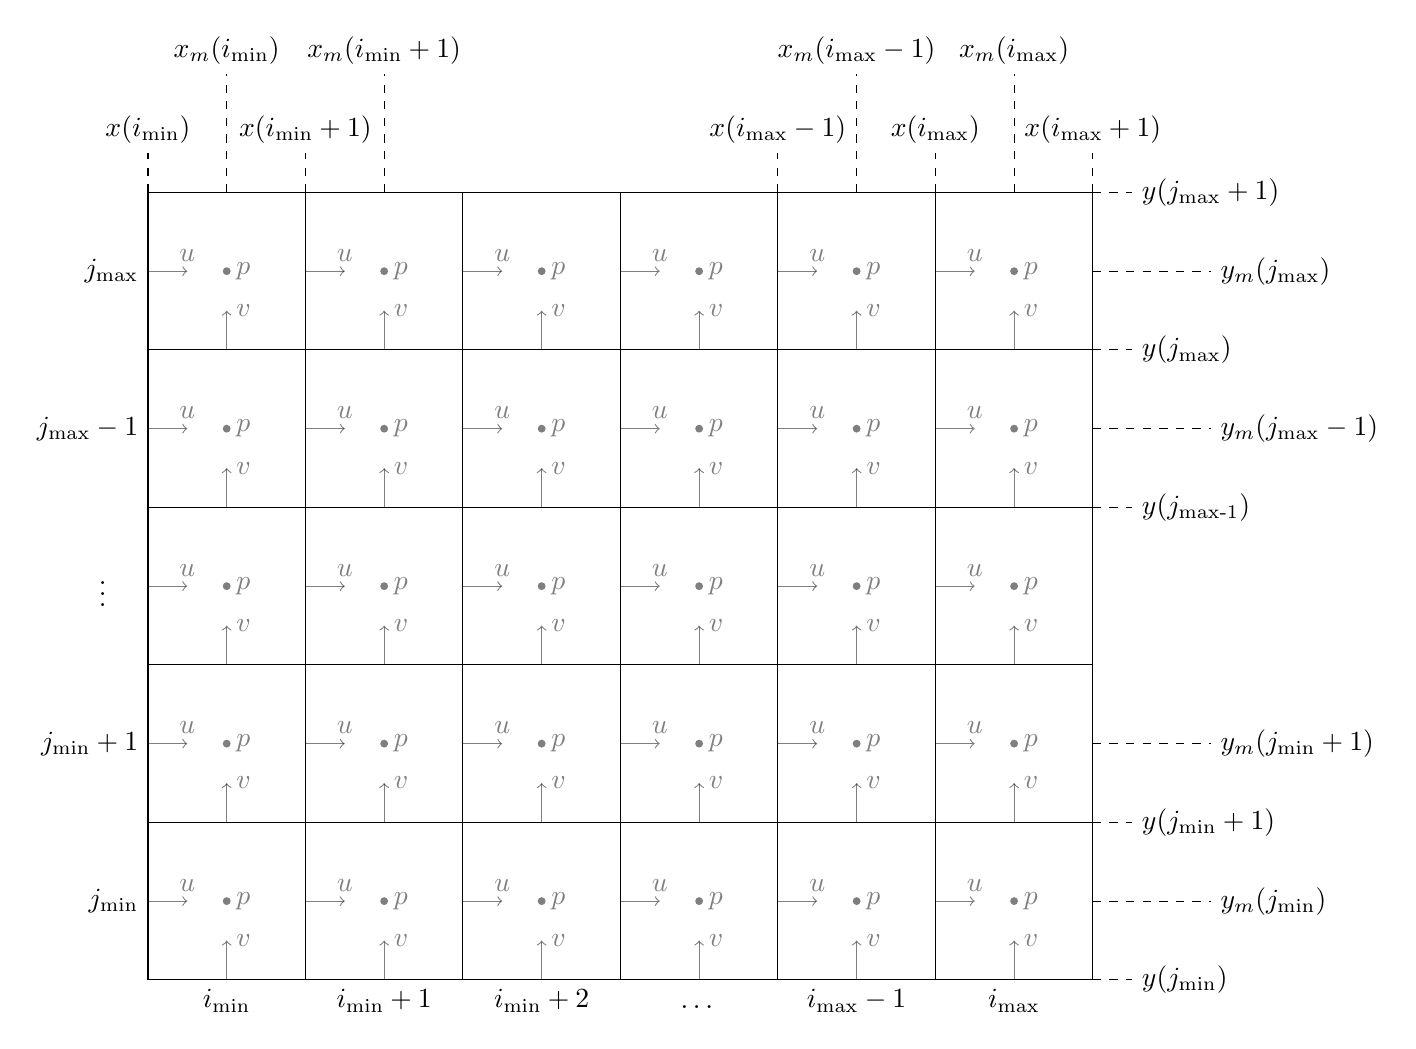
\begin{tikzpicture}[scale=2]
    \draw [] (0,0) grid (6,5);
    \node [anchor=north] at (0.5,0) {$i_\text{min}$};
    \node [anchor=north] at (1.5,0) {$i_\text{min}+1$};
    \node [anchor=north] at (2.5,0) {$i_\text{min}+2$};
    \node [anchor=north] at (3.5,-0.1) {$\dots$};
    \node [anchor=north] at (4.5,0) {$i_\text{max}-1$};
    \node [anchor=north] at (5.5,0) {$i_\text{max}$};

    \node [anchor=east]  at (0,0.5) {$j_\text{min}$};
    \node [anchor=east]  at (0,1.5) {$j_\text{min}+1$};
    \node [anchor=east]  at (-0.2,2.5) {$\vdots$};
    \node [anchor=east]  at (0,3.5) {$j_\text{max}-1$};
    \node [anchor=east]  at (0,4.5) {$j_\text{max}$};

    \foreach \x in {0,...,5}
    {
      \foreach \y in {0,...,4}
      {
        \draw [arrows=->,opacity=0.5] (\x,\y+0.5) -- node[pos=1,above] {$u$} ++(0.25,0);
        \draw [arrows=->,opacity=0.5] (\x+0.5,\y) -- node[pos=1,right] {$v$} ++(0,0.25);
        \fill [opacity=0.5] (\x+0.5,\y+0.5) circle [radius=0.025] node[right] {$p$};
      }
    }
   
    \draw [dashed] (0,5) -- node[pos=1,above] {$x(i_\text{min})$} ++ (0,0.25);
    \draw [dashed] (1,5) -- node[pos=1,above] {$x(i_\text{min}+1)$} ++ (0,0.25);
    \draw [dashed] (4,5) -- node[pos=1,above] {$x(i_\text{max}-1)$} ++ (0,0.25);
    \draw [dashed] (5,5) -- node[pos=1,above] {$x(i_\text{max})$} ++ (0,0.25);
    \draw [dashed] (6,5) -- node[pos=1,above] {$x(i_\text{max}+1)$} ++ (0,0.25);

    \draw [dashed] (0.5,5) -- node[pos=1,above] {$x_m(i_\text{min})$} ++ (0,0.75);
    \draw [dashed] (1.5,5) -- node[pos=1,above] {$x_m(i_\text{min}+1)$} ++ (0,0.75);
    \draw [dashed] (4.5,5) -- node[pos=1,above] {$x_m(i_\text{max}-1)$} ++ (0,0.75);
    \draw [dashed] (5.5,5) -- node[pos=1,above] {$x_m(i_\text{max})$} ++ (0,0.75);

    \draw [dashed] (6,0) -- node[pos=1,right] {$y(j_\text{min})$} ++ (0.25,0);
    \draw [dashed] (6,1) -- node[pos=1,right] {$y(j_\text{min}+1)$} ++ (0.25,0);
    \draw [dashed] (6,3) -- node[pos=1,right] {$y(j_\text{max-1})$} ++ (0.25,0);
    \draw [dashed] (6,4) -- node[pos=1,right] {$y(j_\text{max})$} ++ (0.25,0);
    \draw [dashed] (6,5) -- node[pos=1,right] {$y(j_\text{max}+1)$} ++ (0.25,0);

    \draw [dashed] (6,0.5) -- node[pos=1,right] {$y_m(j_\text{min})$} ++ (0.75,0);
    \draw [dashed] (6,1.5) -- node[pos=1,right] {$y_m(j_\text{min}+1)$} ++ (0.75,0);
    \draw [dashed] (6,3.5) -- node[pos=1,right] {$y_m(j_\text{max}-1)$} ++ (0.75,0);
    \draw [dashed] (6,4.5) -- node[pos=1,right] {$y_m(j_\text{max})$} ++ (0.75,0);

    % \draw [dashed,red] (1.5,3) |- (2.5,4) |- cycle;
    % \node[anchor=south,red] at (1.5,4) {$u$ cell};

    % \draw [dashed,blue] (3,1.5) |- (4,2.5) |- cycle;
    % \node[anchor=west,blue] at (4,1.5) {$v$ cell};


  \end{tikzpicture}
  \caption{Computational mesh with location of the velocities and pressures.  The $x$, $x_m$, $y$, and $y_m$ array locations are also shown.}
  \label{fig:mesh}
\end{figure}

\clearpage
\section{Temporal discretization}
Temporal discretization is done using an explicit Euler scheme which can be written as,
\begin{equation}\label{eq:timedisc}
  \frac{\bm{u}^{n+1}-\bm{u}^n}{\Delta t} = -\frac{1}{\rho}\nabla p^{n+1} -\bm{u}^n\cdot\nabla\bm{u}^n + \nu\nabla^2\bm{u}^n.
\end{equation}
In the previous equation the superscript refers to the temporal iteration.  Typically the simulation is started with $n=0$ and the initial condition is used to populate the initial velocity field $\bm{u}^{n=0}$.  The equation is used to find subsequent solutions.  The time-step $\Delta t$ should be chosen so that $u \Delta t/\Delta x < 1$.  This condition is known as the Courant-Friedrichs-Lewy (CFL) condition.

The previous equation does not include the role of continuity and $u^{n+1}$ is not guaranteed to be divergence-free.  To introduce continuity we solve this equation using the predictor-corrector or fractional step methodology.  In this framework the Navier-Stokes equations are solved in two steps.  

The first step, known as the \emph{predictor step}, is to compute an intermediate velocity $\bm{u}^*$ by solving the momentum equation but omitting the effect of pressure, \ie,
\begin{equation}\label{eq:pred}
  \frac{\bm{u}^*-\bm{u}^n}{\Delta t} = -\bm{u}^n\cdot\nabla\bm{u}^n + \nu\nabla^2\bm{u}^n.
\end{equation}

The second step, known as the \emph{corrector step}, is to solve for the new velocity $u^{n+1}$ and include the influence of the pressure leading to
\begin{equation}\label{eq:corr}
  \frac{\bm{u}^{n+1}-\bm{u}^*}{\Delta t}=-\frac{1}{\rho}\nabla p^{n+1}.
\end{equation}
It is easy to show that Eq.~\ref{eq:timedisc} = Eq.~\ref{eq:pred} + Eq.~\ref{eq:corr}.

The pressure is found such that $u^{n+1}$ satisfies the continuity equation by solving
\begin{equation}\label{eq:Poisson}
  \nabla^2p^{n+1}=\frac{\rho}{\Delta t} \nabla\cdot\bm{u}^*,
\end{equation}
which can be derived by taking the divergence of Eq.~\ref{eq:corr} and enforcing $\nabla\cdot\bm{u}^{n+1}=0$.  This equation is referred to as the \emph{pressure Poisson equation}.


\section{$u$ momentum discretization}\label{sec:u}

The convective and viscous terms in Eq.~\ref{eq:pred} are discretized using finite differences which approximate the derivatives using neighboring values.


The predictor step for $u$ velocity can be written as
\begin{equation}
  u^*=u^n+\Delta t\left(\nu\left(\frac{\partial^2u^n}{\partial x^2}+\frac{\partial^2u^n}{\partial y^2}\right) 
  -\left(u^n\frac{\partial u^n}{\partial x}+v^n\frac{\partial u^n}{\partial y}\right)\right)
\end{equation}
The viscous and convective terms are discretized for the $i,j$ cell using
\begin{align}
  \frac{\partial^2 u}{\partial x^2} &= \frac{u(i-1,j)-2u(i,j)+u(i+1,j)}{\Delta x^2} \\
  \frac{\partial^2 u}{\partial y^2} &= \frac{u(i,j-1)-2u(i,j)+u(i,j+1)}{\Delta y^2} \\
  u\frac{\partial u}{\partial x} &= u(i,j)\frac{u(i+1,j)-u(i-1,j)}{2\Delta x}\\
  v\frac{\partial u}{\partial y} &= \frac{1}{4}\left(v(i-1,j)+v(i,j)+v(i-1,j+1)+v(i,j+1)\right)\frac{u(i,j+1)-u(i,j-1)}{2\Delta y}
\end{align}

Figure~\ref{fig:ucell} shows the velocity values used in the discretization.

\begin{figure}[htbp]
  \centering
  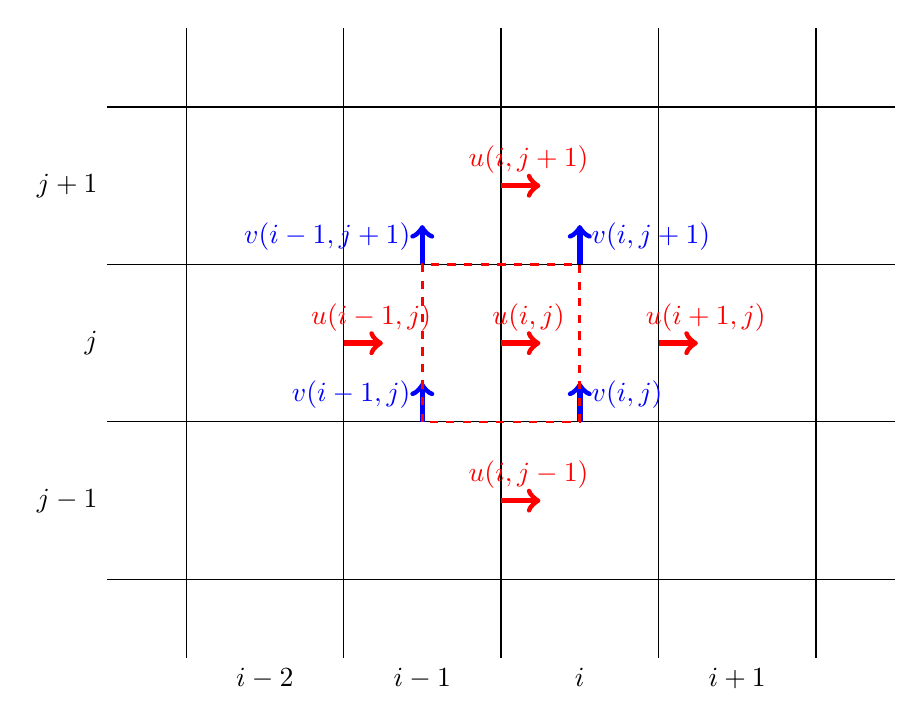
\begin{tikzpicture}[scale=2]
    \draw [] (0.5,0.5) grid (5.5,4.5);
    \node [anchor=north] at (1.5,0.5) {$i-2$};
    \node [anchor=north] at (2.5,0.5) {$i-1$};
    \node [anchor=north] at (3.5,0.5) {$i$};
    \node [anchor=north] at (4.5,0.5) {$i+1$};

    \node [anchor=east]  at (0.5,1.5) {$j-1$};
    \node [anchor=east]  at (0.5,2.5) {$j$};
    \node [anchor=east]  at (0.5,3.5) {$j+1$};

    \draw [arrows=->,line width=2,red] (2,2.5) -- node[pos=0.7,above] {$u(i-1,j)$} ++(0.25,0);
    \draw [arrows=->,line width=2,red] (3,2.5) -- node[pos=0.7,above] {$u(i,j)$} ++(0.25,0);
    \draw [arrows=->,line width=2,red] (3,3.5) -- node[pos=0.7,above] {$u(i,j+1)$} ++(0.25,0);
    \draw [arrows=->,line width=2,red] (3,1.5) -- node[pos=0.7,above] {$u(i,j-1)$} ++(0.25,0);
    \draw [arrows=->,line width=2,red] (4,2.5) -- node[pos=1.2,above] {$u(i+1,j)$} ++(0.25,0);

    \draw [arrows=->,line width=2,blue] (2.5,2) -- node[pos=0.7,left] {$v(i-1,j)$} ++(0,0.25);
    \draw [arrows=->,line width=2,blue] (3.5,2) -- node[pos=0.7,right] {$v(i,j)$} ++(0,0.25);
    \draw [arrows=->,line width=2,blue] (3.5,3) -- node[pos=0.7,right] {$v(i,j+1)$} ++(0,0.25);
    \draw [arrows=->,line width=2,blue] (2.5,3) -- node[pos=0.7,left] {$v(i-1,j+1)$} ++(0,0.25);

    \draw [dashed,red,line width=1] (2.5,2) |- (3.5,3) |- cycle;


  \end{tikzpicture}
  \caption{Velocities and their locations used to discretize the $u(i,j)$ cell in the $u$-momentum equation..}
  \label{fig:ucell}
\end{figure}

\begin{figure}[htbp]
  \centering
  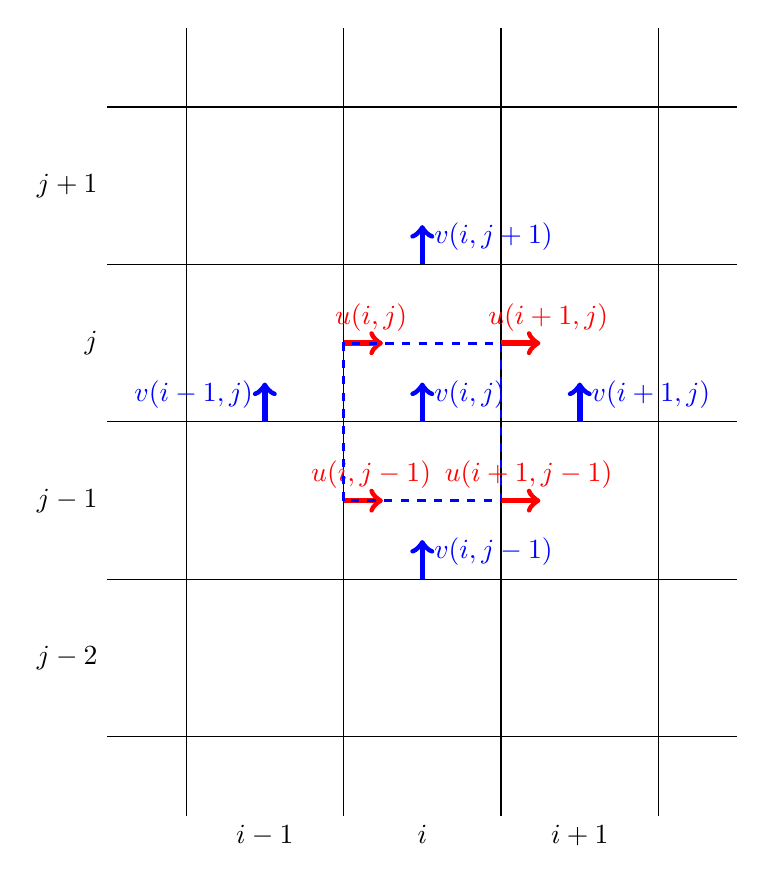
\begin{tikzpicture}[scale=2]
    \draw [] (1.5,-0.5) grid (5.5,4.5);
    \node [anchor=north] at (2.5,-0.5) {$i-1$};
    \node [anchor=north] at (3.5,-0.5) {$i$};
    \node [anchor=north] at (4.5,-0.5) {$i+1$};

    \node [anchor=east]  at (1.5,0.5) {$j-2$};
    \node [anchor=east]  at (1.5,1.5) {$j-1$};
    \node [anchor=east]  at (1.5,2.5) {$j$};
    \node [anchor=east]  at (1.5,3.5) {$j+1$};

    \draw [arrows=->,line width=2,red] (3,2.5) -- node[pos=0.7,above] {$u(i,j)$} ++(0.25,0);
    \draw [arrows=->,line width=2,red] (3,1.5) -- node[pos=0.7,above] {$u(i,j-1)$} ++(0.25,0);
    \draw [arrows=->,line width=2,red] (4,2.5) -- node[pos=1.2,above] {$u(i+1,j)$} ++(0.25,0);
    \draw [arrows=->,line width=2,red] (4,1.5) -- node[pos=0.7,above] {$u(i+1,j-1)$} ++(0.25,0);

    \draw [arrows=->,line width=2,blue] (2.5,2) -- node[pos=0.7,left] {$v(i-1,j)$} ++(0,0.25);
    \draw [arrows=->,line width=2,blue] (3.5,2) -- node[pos=0.7,right] {$v(i,j)$} ++(0,0.25);
    \draw [arrows=->,line width=2,blue] (3.5,3) -- node[pos=0.7,right] {$v(i,j+1)$} ++(0,0.25);
    \draw [arrows=->,line width=2,blue] (3.5,1) -- node[pos=0.7,right] {$v(i,j-1)$} ++(0,0.25);
    \draw [arrows=->,line width=2,blue] (4.5,2) -- node[pos=0.7,right] {$v(i+1,j)$} ++(0,0.25);

    \draw [dashed,blue,line width=1] (3,1.5) |- (4,2.5) |- cycle;


  \end{tikzpicture}
  \caption{Velocities and their locations used to discretize the $v(i,j)$ cell in the $v$-momentum equation..}
  \label{fig:vcell}
\end{figure}

MATLAB code that computes $u^*$ is
\begin{lstlisting}
    for j=jmin:jmax
        for i=imin+1:imax
            v_here=0.25*(v(i-1,j)+v(i-1,j+1)+v(i,j)+v(i,j+1));
            us(i,j)=u(i,j)+dt* ...
                (nu*(u(i-1,j)-2*u(i,j)+u(i+1,j))*dxi^2 ...
                +nu*(u(i,j-1)-2*u(i,j)+u(i,j+1))*dyi^2 ...
                -u(i,j)*(u(i+1,j)-u(i-1,j))*0.5*dxi ...
                -v_here*(u(i,j+1)-u(i,j-1))*0.5*dyi);
        end
    end
  \end{lstlisting}

\section{$v$ momentum discretization}\label{sec:v}

Following the same approach as we did for $u$ we can write the predictor step for the $v$ velocity as
\begin{equation}
  v^*=v^n+\Delta t\left(\nu\left(\frac{\partial^2v^n}{\partial x^2}+\frac{\partial^2v^n}{\partial y^2}\right) 
  -\left(u\frac{\partial v^n}{\partial x}+v^n\frac{\partial v^n}{\partial y}\right)\right).
\end{equation}
The viscous and convective terms are discretized for the $i,j$ cell using
\begin{align}
  \frac{\partial^2 v}{\partial x^2} &= \frac{v(i-1,j)-2v(i,j)+v(i+1,j)}{\Delta x^2}  \\
  \frac{\partial^2 v}{\partial y^2} &= \frac{v(i,j-1)-2v(i,j)+v(i,j+1)}{\Delta y^2} \\
  u\frac{\partial v}{\partial x} &= \frac{1}{4}\left(u(i,j-1)+u(i,j)+u(i+1,j-1)+u(i+1,j)\right)\frac{v(i+1,j)-v(i-1,j)}{2\Delta x}\\
  v\frac{\partial v}{\partial y} &= v(i,j)\frac{v(i,j+1)-v(i,j-1)}{2\Delta y}
\end{align}

Figure~\ref{fig:vcell} shows the velocity values used in the discretization.

MATLAB code that computes $v^*$ is
\begin{lstlisting}
    for j=jmin+1:jmax
        for i=imin:imax
            u_here=0.25*(u(i,j-1)+u(i,j)+u(i+1,j-1)+u(i+1,j));
            vs(i,j)=v(i,j)+dt* ...
                (nu*(v(i-1,j)-2*v(i,j)+v(i+1,j))*dxi^2 ...
                +nu*(v(i,j-1)-2*v(i,j)+v(i,j+1))*dyi^2 ...
                -u_here*(v(i+1,j)-v(i-1,j))*0.5*dxi ...
                -v(i,j)*(v(i,j+1)-v(i,j-1))*0.5*dyi);
        end
    end
\end{lstlisting}

\newpage
\section{Poisson equation}\label{sec:poisson}
The pressure Poisson equation, Eq.~\ref{eq:Poisson} is used to create a velocity field that satisfies the continuity equation and is incompressible.  Solving the Poisson equation almost always uses the majority of the computational cost in the solution calculation.  Many ways can be used to solve the Poisson equation and some are faster than others.  The simplest way to solve the Poisson equation is to write it as 
\begin{equation}\label{eq:PoissonMatrix}
  \bm{L}\bm{p}^{n+1}=\bm{R}
\end{equation}
where $\bm{L}=\nabla^2$ is the Laplacian operator (a large $n_x\cdot n_y \times n_x\cdot n_y$ matrix), $\bm{p}^{n+1}$ is the pressure in each computational cell organized into one large vector, and $\bm{R}=-\frac{\rho}{\Delta t}\nabla\cdot\bm{u}^*$ is the right-hand-side of the pressure Poisson equation in each computational cell organized into one large vector.  This equation can be solved for $\bm{p}^{n+1}$ using MATLAB's built in solver, \ie, $\bm{p}^{n+1}=\bm{L}\backslash \bm{R}$.  It is advisable to use this method in your first CFD code.  Note that there are other methods that do not require forming $\bm{L}$ which requires too much memory to store for large problems.  

Boundary conditions for the Pressure poisson equation are Neuman or zero derivative.  Additionally, the pressure poisson equation is only defined up to a constant and the pressure in one computational cell needs to be set.  All other pressures in the domain are computed with respect to this pressure.  

To discretie the pressure equation in the $i,j$ cell we use (see Fig.~\ref{fig:pcell} for details on the location of pressures and velocities),
\begin{align}
\nabla^2 p^{n+1} &= \frac{\partial^2 p^{n+1}}{\partial x^2} +\frac{\partial^2 p^{n+1}}{\partial y^2} \nonumber\\
&\approx \frac{p^{n+1}(i-1,j)-2p^{n+1}(i,j)+p^{n+1}(i+1,j)}{\Delta x^2} + \frac{p^{n+1}(i,j-1)-2p^{n+1}(i,j)+p^{n+1}(i,j+1)}{\Delta y^2}\label{eq:Lap}\\
\nabla\cdot\bm{u}^*&=\frac{\partial u^*}{\partial x} + \frac{\partial v^*}{\partial y} \nonumber\\
& \approx \frac{u^*(i+1,j)-u^*(i,j)}{\Delta x} + \frac{v^*(i,j+1)-v^*(i,j)}{\Delta y}
\end{align}

Using this discretization we can write Eq.~\ref{eq:PoissonMatrix} as
\begin{equation}
  \begin{array}{cccc}
    \bm{L}&\bm{p}^{n+1}&=&\bm{R} \\
    ~\\
    \renewcommand{\arraystretch}{2}
    \begin{bmatrix*}[r]
      1  &   0  &    0  &   0  &    0  &    0  &    0  &    0  &    0\\
      \frac{-1}{\Delta x^2}  &    D_y  &   \frac{-1}{\Delta x^2}  &    0  &   \frac{-1}{\Delta y^2}  &    0  &    0  &    0  &    0\\
      0  &   \frac{-1}{\Delta x^2}  &    D_{xy}  &    0  &    0  &   \frac{-1}{\Delta y^2}  &    0  &    0  &    0\\
      \frac{-1}{\Delta y^2}  &    0  &    0  &    D_x  &   \frac{-1}{\Delta x^2}  &    0  &   \frac{-1}{\Delta y^2}  &    0  &    0\\
      0  &   \frac{-1}{\Delta y^2}  &    0  &   \frac{-1}{\Delta x^2}  &    D  &   \frac{-1}{\Delta x^2}  &    0  &   \frac{-1}{\Delta y^2}  &    0\\
      0  &    0  &   \frac{-1}{\Delta y^2}  &    0  &   \frac{-1}{\Delta x^2}  &    D_x  &    0  &    0  &   \frac{-1}{\Delta y^2}\\
      0  &    0  &    0  &   \frac{-1}{\Delta y^2}  &    0  &    0  &    D_{xy}  &   \frac{-1}{\Delta x^2}  &    0\\
      0  &    0  &    0  &    0  &   \frac{-1}{\Delta y^2}  &    0  &   \frac{-1}{\Delta x^2}  &    D_{y}  &   \frac{-1}{\Delta x^2}\\
      0  &    0  &    0  &    0  &    0  &   \frac{-1}{\Delta y^2}  &    0  &   \frac{-1}{\Delta x^2}  &    D_{xy}\\
    \end{bmatrix*} &
    \renewcommand{\arraystretch}{2}
    \begin{bmatrix}
      p(1,1) \\ p(2,1) \\ p(3,1)\\
      p(1,2) \\ p(2,2) \\ p(3,2)\\
      p(1,3) \\ p(2,3) \\ p(3,3)\\
    \end{bmatrix}&
    =&
    \renewcommand{\arraystretch}{2}
    \begin{bmatrix}
      R(1,1) \\ R(2,1) \\ R(3,1)\\
      R(1,2) \\ R(2,2) \\ R(3,2)\\
      R(1,3) \\ R(2,3) \\ R(3,3)\\
    \end{bmatrix}
  \end{array}
\end{equation}
where $D=\frac{2}{\Delta x^2}+\frac{2}{\Delta y^2}$, $D_x=D-\frac{1}{\Delta x^2}$, $D_y=D-\frac{1}{\Delta y^2}$, and $D_{xy}=D-\frac{1}{\Delta x^2} - \frac{1}{\Delta y^2}$.  The modify diagonal entries are due to the Neuman boundary conditions. For this $n_x\times n_y=3\times3$ problem there is only 1 interior point and the unmodified $D$ only shows up once. 

 Note that the Laplacian only depends on the computational mesh and can be computed once at the beginning of the simulation and stored.  Additionally you can greatly speed-up your code by performing an LU decomposition of $L$ which can easily be done in MATLAB using \lstinline{L = decomposition(L);}. Here is MATLAB code that creates the Laplacian operator $\bm{L}$:

\noindent\begin{minipage}{\linewidth}
\begin{lstlisting}
    % Create Laplacian operator for solving pressure Poisson equation 
    L=zeros(nx*ny,nx*ny);
    for j=1:ny
        for i=1:nx
            L(i+(j-1)*nx,i+(j-1)*nx)=2*dxi^2+2*dyi^2;
            for ii=i-1:2:i+1
                if (ii>0 && ii<=nx) % Interior point
                    L(i+(j-1)*nx,ii+(j-1)*nx)=-dxi^2;
                else                % Neuman conditions on boundary
                    L(i+(j-1)*nx,i +(j-1)*nx)= ...
                        L(i+(j-1)*nx,i +(j-1)*nx)-dxi^2;
                end
            end
            for jj=j-1:2:j+1
                if (jj>0 && jj<=ny) % Interior point
                    L(i+(j-1)*nx,i+(jj-1)*nx)=-dyi^2;
                else                % Neuman conditions on boundary
                    L(i+(j-1)*nx,i+(j -1)*nx)= ...
                        L(i+(j-1)*nx,i+(j -1)*nx)-dyi^2;
                end
            end
        end
    end
    % Set pressure in first cell (all other pressures w.r.t to this one)
    L(1,:)=0; L(1,1)=1;

    % Perform LU decomposition to speed-up code (uncomment once code is working)
    % L = decomposition(L);
\end{lstlisting}
\end{minipage}

MATLAB code to compute the right-hand-side $\bm{R}$ is:
\begin{lstlisting}
    n=0;
    for j=jmin:jmax
        for i=imin:imax 
            n=n+1;
            R(n)=-rho/dt* ...
                ((us(i+1,j)-us(i,j))*dxi ...
                +(vs(i,j+1)-vs(i,j))*dyi);
        end
    end
\end{lstlisting}

The pressure is found by solving $\bm{L}\bm{p}^{n+1}=\bm{R}$ which in MATLAB can be done using
\begin{lstlisting}
    pv=L\R;
\end{lstlisting}
where \lstinline{pv} is the vector representation of the pressure.  Finally, \lstinline{pv} is converted to the mesh representation \lstinline{p(i,j)} which can be done using
\begin{lstlisting}
    n=0;
    p=zeros(imax,jmax);
    for j=jmin:jmax
        for i=imin:imax
            n=n+1;
            p(i,j)=pv(n);
        end
    end
\end{lstlisting}


\begin{figure}[htbp]
  \centering
  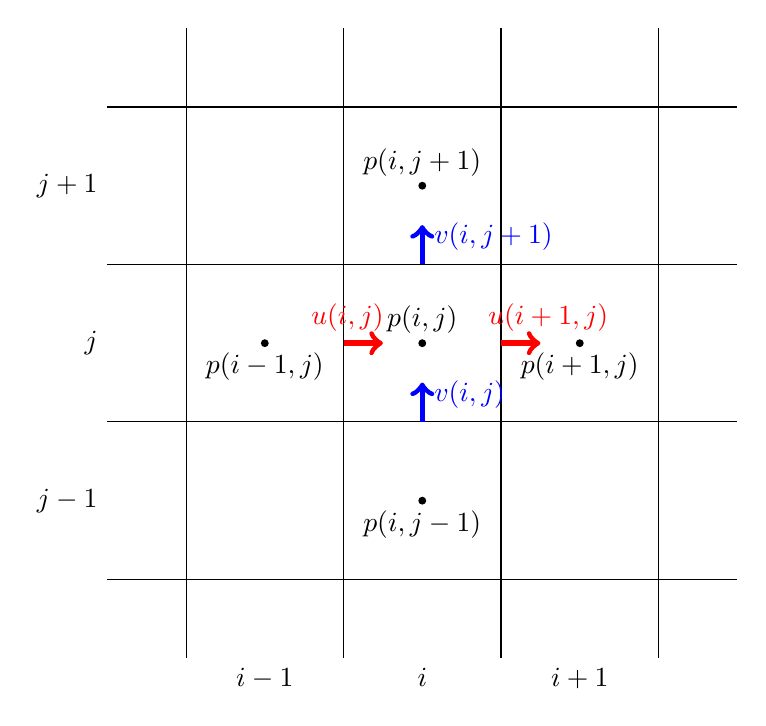
\begin{tikzpicture}[scale=2]
    \draw [] (1.5,0.5) grid (5.5,4.5);
    \node [anchor=north] at (2.5,0.5) {$i-1$};
    \node [anchor=north] at (3.5,0.5) {$i$};
    \node [anchor=north] at (4.5,0.5) {$i+1$};

    \node [anchor=east]  at (1.5,1.5) {$j-1$};
    \node [anchor=east]  at (1.5,2.5) {$j$};
    \node [anchor=east]  at (1.5,3.5) {$j+1$};

    \fill [] (3.5,2.5) circle [radius=0.025] node[above] {$p(i,j)$};
    \fill [] (4.5,2.5) circle [radius=0.025] node[below] {$p(i+1,j)$};
    \fill [] (2.5,2.5) circle [radius=0.025] node[below] {$p(i-1,j)$};
    \fill [] (3.5,1.5) circle [radius=0.025] node[below] {$p(i,j-1)$};
    \fill [] (3.5,3.5) circle [radius=0.025] node[above] {$p(i,j+1)$};

    \draw [arrows=->,line width=2,red] (3,2.5) -- node[pos=0.1,above] {$u(i,j)$} ++(0.25,0);
    \draw [arrows=->,line width=2,red] (4,2.5) -- node[pos=1.2,above] {$u(i+1,j)$} ++(0.25,0);
    \draw [arrows=->,line width=2,blue] (3.5,2) -- node[pos=0.7,right] {$v(i,j)$} ++(0,0.25);
    \draw [arrows=->,line width=2,blue] (3.5,3) -- node[pos=0.7,right] {$v(i,j+1)$} ++(0,0.25);
  \end{tikzpicture}
  \caption{Velocities and their locations used to discretize the $p(i,j)$ cell in the pressure Poisson equation.}
  \label{fig:pcell}
\end{figure}

\section{Corrector step}\label{sec:corr}
Once the pressure is computed using the Poisson equation it is used to update the velocity from $\bm{u}^*$ to $\bm{u}^{n+1}$ using Eq.~\ref{eq:corr}.
The pressure gradient can be computed using finite differences.  To update $u$ and $v$ we use
\begin{align}
  \frac{\partial p}{\partial x}&=\frac{p(i,j)-p(i-1,j)}{\Delta x},\text{ and}\\
  \frac{\partial p}{\partial y}&=\frac{p(i,j)-p(i,j-1)}{\Delta y},
\end{align}
respectively.  MATLAB code to perform the corrector step is:
\begin{lstlisting}
    for j=jmin:jmax
        for i=imin+1:imax
            u(i,j)=us(i,j)-dt/rho*(p(i,j)-p(i-1,j))*dxi;
        end
    end
    for j=jmin+1:jmax
        for i=imin:imax
            v(i,j)=vs(i,j)-dt/rho*(p(i,j)-p(i,j-1))*dyi;
        end
    end
\end{lstlisting}

\newpage
\section{Boundary conditions}\label{sec:BC}

Boundary conditions are needed for the velocity field and the pressure Poisson equation.  The velocity boundary conditions are a bit tricky since some of the velocity components are not defined on the boundary.  For example, to specify $u=u_\text{top}$ at the top of the domain is not straightforward because $u$ is defined $\Delta x/2$ away from the top boundary.  One solution to this problem is to create a fictitious velocity outside the domain such that the velocity on the domain boundary satisfies the boundary condition.  In Fig.~\ref{fig:BC} shows how using a fictitious velocity at $u(i,j_\text{max}+1)=-u(i,j_\text{max})$ provides a $u_\text{top}=0$ boundary condition.  For a general boundary condition we can write
\begin{equation}
  u_\text{top} = \frac{1}{2}\left(u(i,j_\text{max})+u(i,j_\text{max}+1)\right),
\end{equation}
which says the velocity at the top of the domain should be the average of the two neighboring velocities (linear interpolation).  Rearranging this equations provides an expression to set the fictitious velocity.
\begin{equation}
  u(i,j_\text{max}+1) = 2 u_\text{top} - u(i,j_\text{max})
\end{equation}
Similar boundary conditions can be written for the other sides of the domain when the velocity is not coincident with the domain boundary.  Here is MATLAB code to enforce the boundary conditions on the four sides of the domain:
\begin{lstlisting}
    u(:,jmin-1)=2*u_bot - u(:,jmin);
    u(:,jmax+1)=2*u_top - u(:,jmax);
    v(imin-1,:)=2*v_lef - v(imin,:);
    v(imax+1,:)=2*v_rig - v(imax,:);
\end{lstlisting}

\begin{figure}[H]
  \centering
  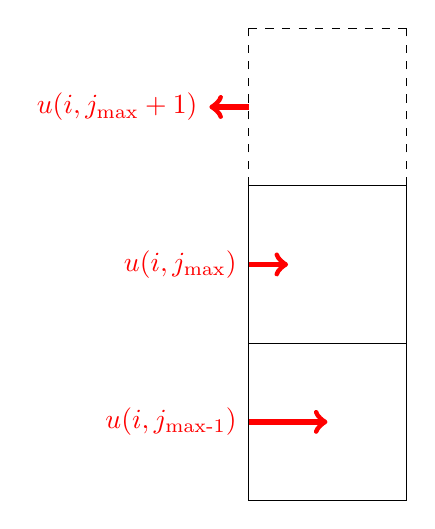
\begin{tikzpicture}[scale=2]
    \draw[] (0,0) grid (1,2);
    \draw[dashed] (0,2) grid (1,3);
    \draw [arrows=->,line width=2,red] (0,2.5) -- node[pos=1.0,left] {$u(i,j_\text{max}+1)$} ++(-0.25,0);
    \draw [arrows=->,line width=2,red] (0,1.5) -- node[pos=0.0,left] {$u(i,j_\text{max})$} ++(0.25,0);
    \draw [arrows=->,line width=2,red] (0,0.5) -- node[pos=0.0,left] {$u(i,j_\text{max-1})$} ++(0.5,0);
  \end{tikzpicture}
  \caption{Example of how to apply a $u_\text{top}=0$ boundary condition using the fictitious velocity $u(i,j_\text{max}+1)$.}
  \label{fig:BC}
\end{figure}

\newpage
\section{General overview of the code}
You've almost made it to the end and are probably overwhelmed by all of the pieces.  In this section, I will try to organize the pieces into a coherent structure that you can use as an outline when you write your code.
\begin{itemize}
\item Set input parameters: viscosity, density, number of grid points, time information, and boundary conditions
\item Create the index extents and the computational grid (see Section~\ref{sec:grid})
\item Initialize any arrays you use to allocate the memory 
\item Create the Laplacian operator (see Section~\ref{sec:poisson})
\item Apply boundary conditions to the initial velocity field (see Section~\ref{sec:BC})
\item Loop over time (use a for or while loop)
  \begin{itemize}
  \item Update time $t=t+\Delta t$
  \item Perform the predictor step to find $u^*$ and $v^*$ (see Sections~\ref{sec:u} and~\ref{sec:v})
  \item Apply boundary conditions to the predicted velocity field (see Section~\ref{sec:BC})
  \item Form the right-hand-side of the Poisson equation (see Section~\ref{sec:poisson})
  \item Solve for the pressure using $\bm{pv}=\bm{L}\backslash \bm{R}$ and convert the pressure vector $pv$ into a matrix $p(i,j)$ (see Section~\ref{sec:poisson})
  \item Perform the corrector step to find $u^{n+1}$ and $v^{n+1}$ (see Section~\ref{sec:corr}) (copy the boundary conditions from the predicted velocity onto $u^{n+1}$ and $v^{n+1}$)
  \item Plot the velocity field and the pressure field
  \end{itemize}
\item End Simulation
\end{itemize}

\section{Test Case}
Once you're code is written, it is useful to test it.  A simple test case to try is the lid-driven cavity problem which is described here: \url{https://www.cfd-online.com/Wiki/Lid-driven_cavity_problem}.

\end{document}
